\section{Durchführung}
\label{sec:Durchführung}

Dieser Versuch wird nur mithilfe des Impuls-Echo-Verfahrens durchgeführt.

\subsection{Versuchsaufbau}
\label{subsec:versuchsaufbau}
In \autoref{fig:echoskop} ist das Ultraschallechoskop zu sehen.
Mithilfe der Ultraschallsonde sollen die Probe untersucht werden, diese ist auf $\SI{2}{\mega\hertz}$ voreingestellt.
Die aufgenommenen Daten des Echoskops werden von einem Rechner erfasst und in einem A-Scan abgebildet.
Die Abszisse beschreibt dabei die Laufzeit $t$ des Impulses in $\si{\micro\second}$, auf der Ordinate wird die Eingangsspannung in Volt angegeben.

\begin{figure}
    \centering
    \includegraphics[width=\textwidth]{content/messgerät.pdf}
    \caption{Das Ultraschallechoskop. Rechts ist die Ultraschallsonde angehängt.\cite{anleitung}}
    \label{fig:echoskop}
\end{figure}

\subsection{Bestimmung der Schallgeschwindigkeit und Untersuchung von Fehlstellen}
\label{aufgabe_1}
Zunächst soll die Schallgeschwindigkeit in Acryl bestimmt werden.
Dafür wird der Acrylblock (siehe \autoref{fig:acrylblock}) sowie die Positionen der Fehlstellen mit der Schieblehre vermessen und mithilfe eines A-Scans untersucht.
Als Kontaktmittel wird hier bidestilliertes Wasser verwendet, da Luft den Ultraschall stark absorbiert.
Zusätzlich steht der Acrylblock auf einem Papiertuch.
Die Kontaktmittel beeinflussen die Messung nicht.
Die Sonde wird auf dem Block über eine Fehlstellen gesetzt.
Die vom Rechner angegebenen Ausschläge werden notiert und die Sonde wird zur nächsten Fehlstelle bewegt.
Dieser Vorgang wird für alle Fehlstellen im Block wiederholt.
Der Block wird gedreht und der gerade beschriebene Messvorgang nochmals wiederholt.

\begin{figure}
    \centering
    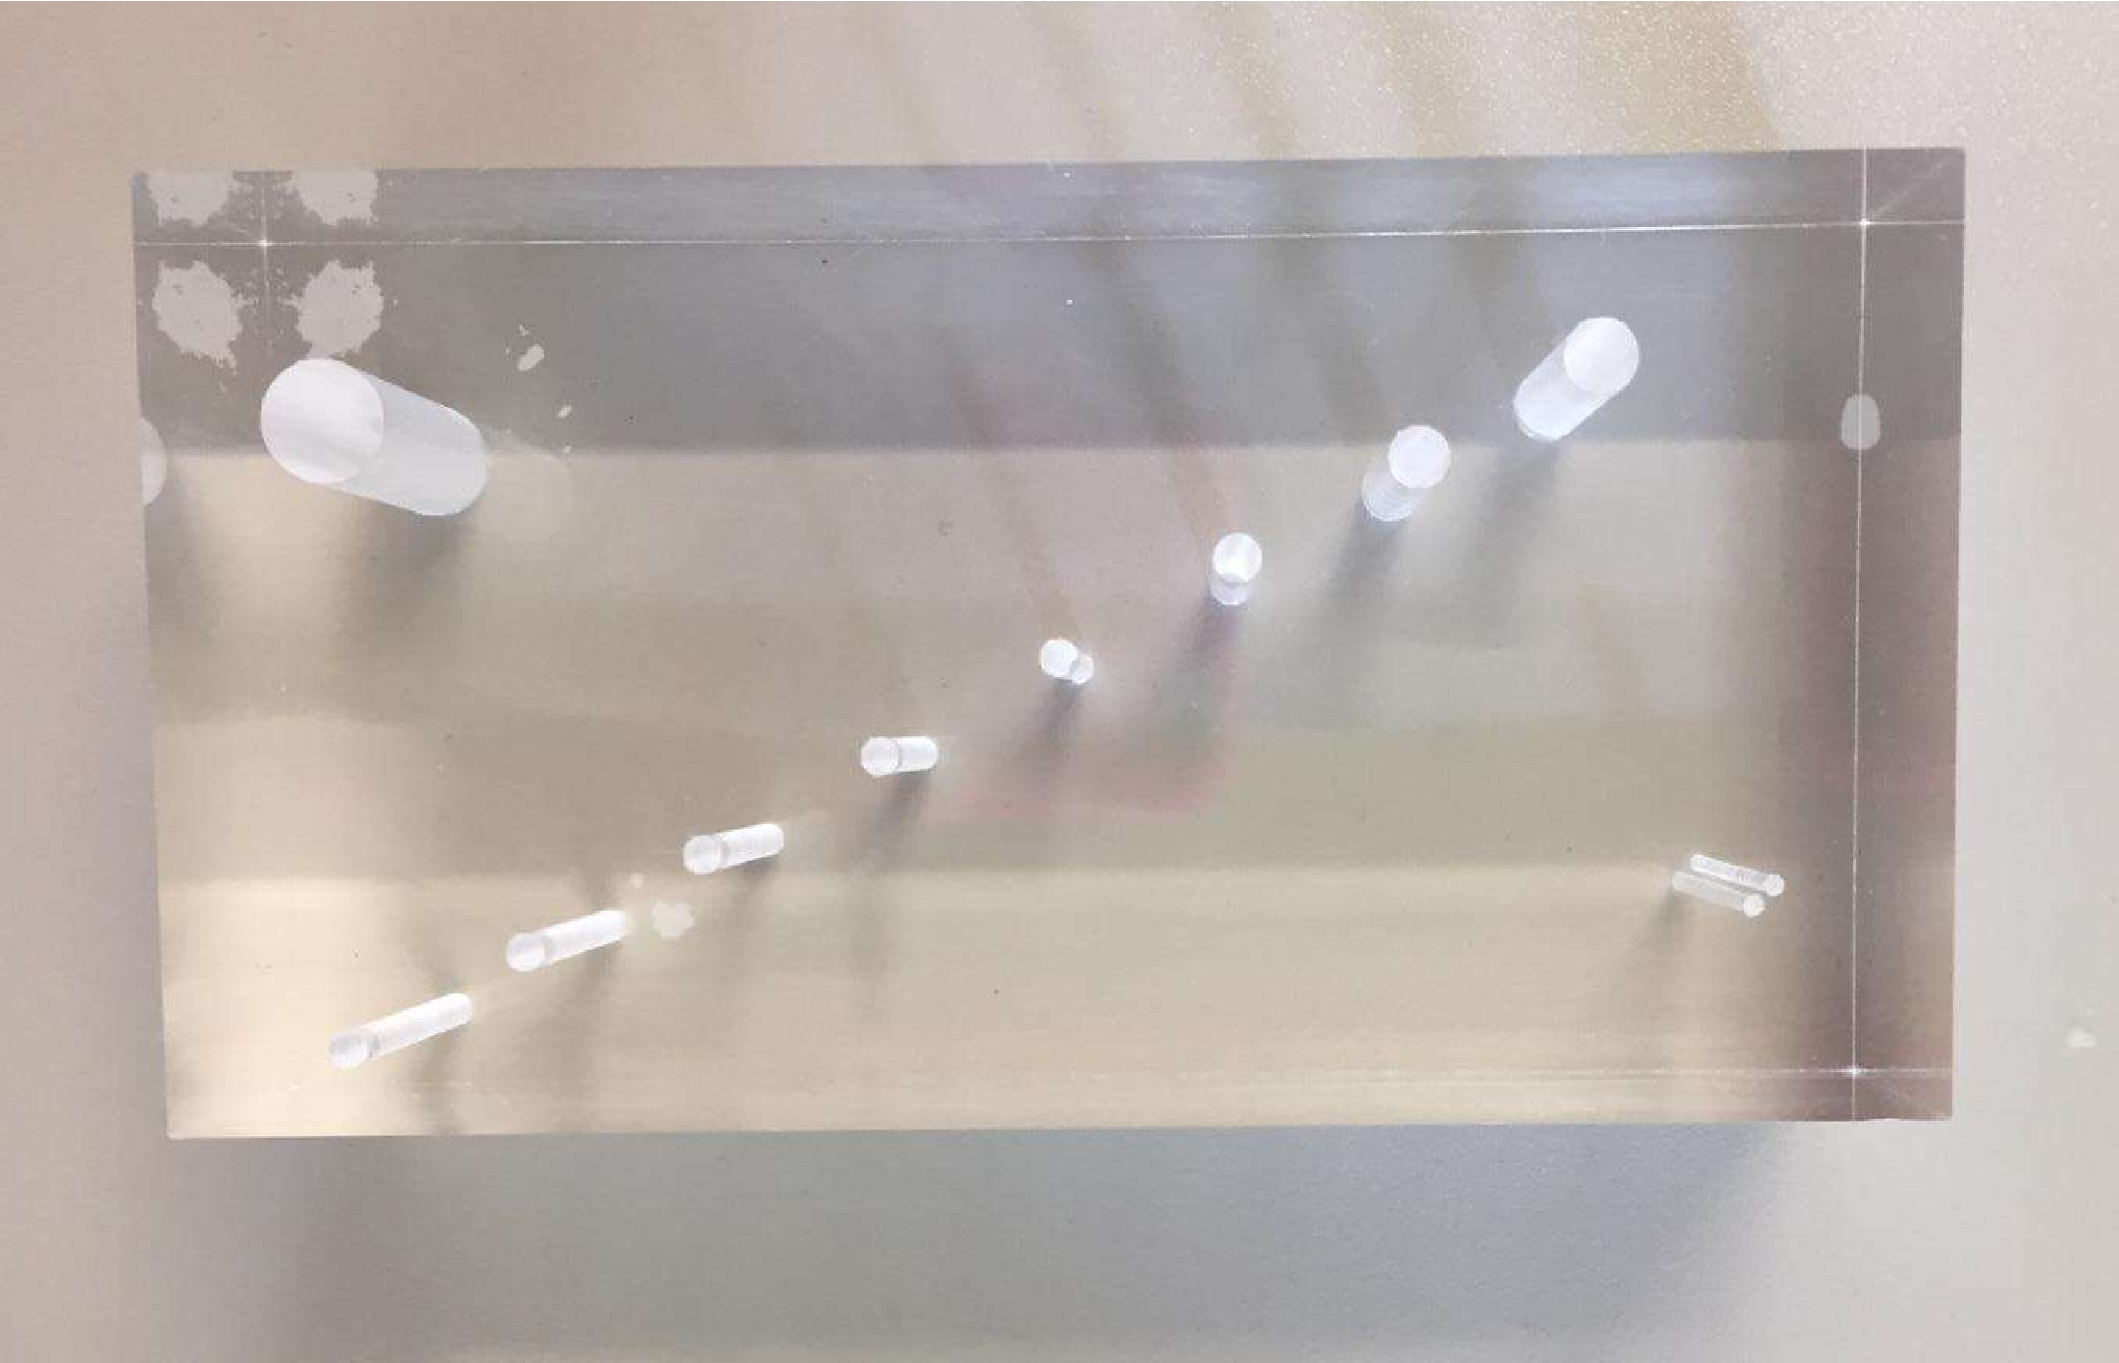
\includegraphics[width=\textwidth]{content/acrylblock.pdf}
    \caption{Der Acrylblock und seine Fehlstellen.}\cite{anleitung}
    \label{fig:acrylblock}
\end{figure}

\subsection{Untersuchung des Augenmodells}
\label{subsec:auge}
Nun soll das Augenmodell (siehe \autoref{fig:auge}) untersucht werden.
Als Kontaktmittel wird ein Koppelgel verwendet.
Die Sonde wird vorsichtig über die Iris bewegt bis auf dem Rechner mehrere Ausschläge zu sehen sind.
Das angezeigte Bild des Rechners wird schnell fotografiert und einige Messwerte werden aufgenommen.

\begin{figure}
    \centering
    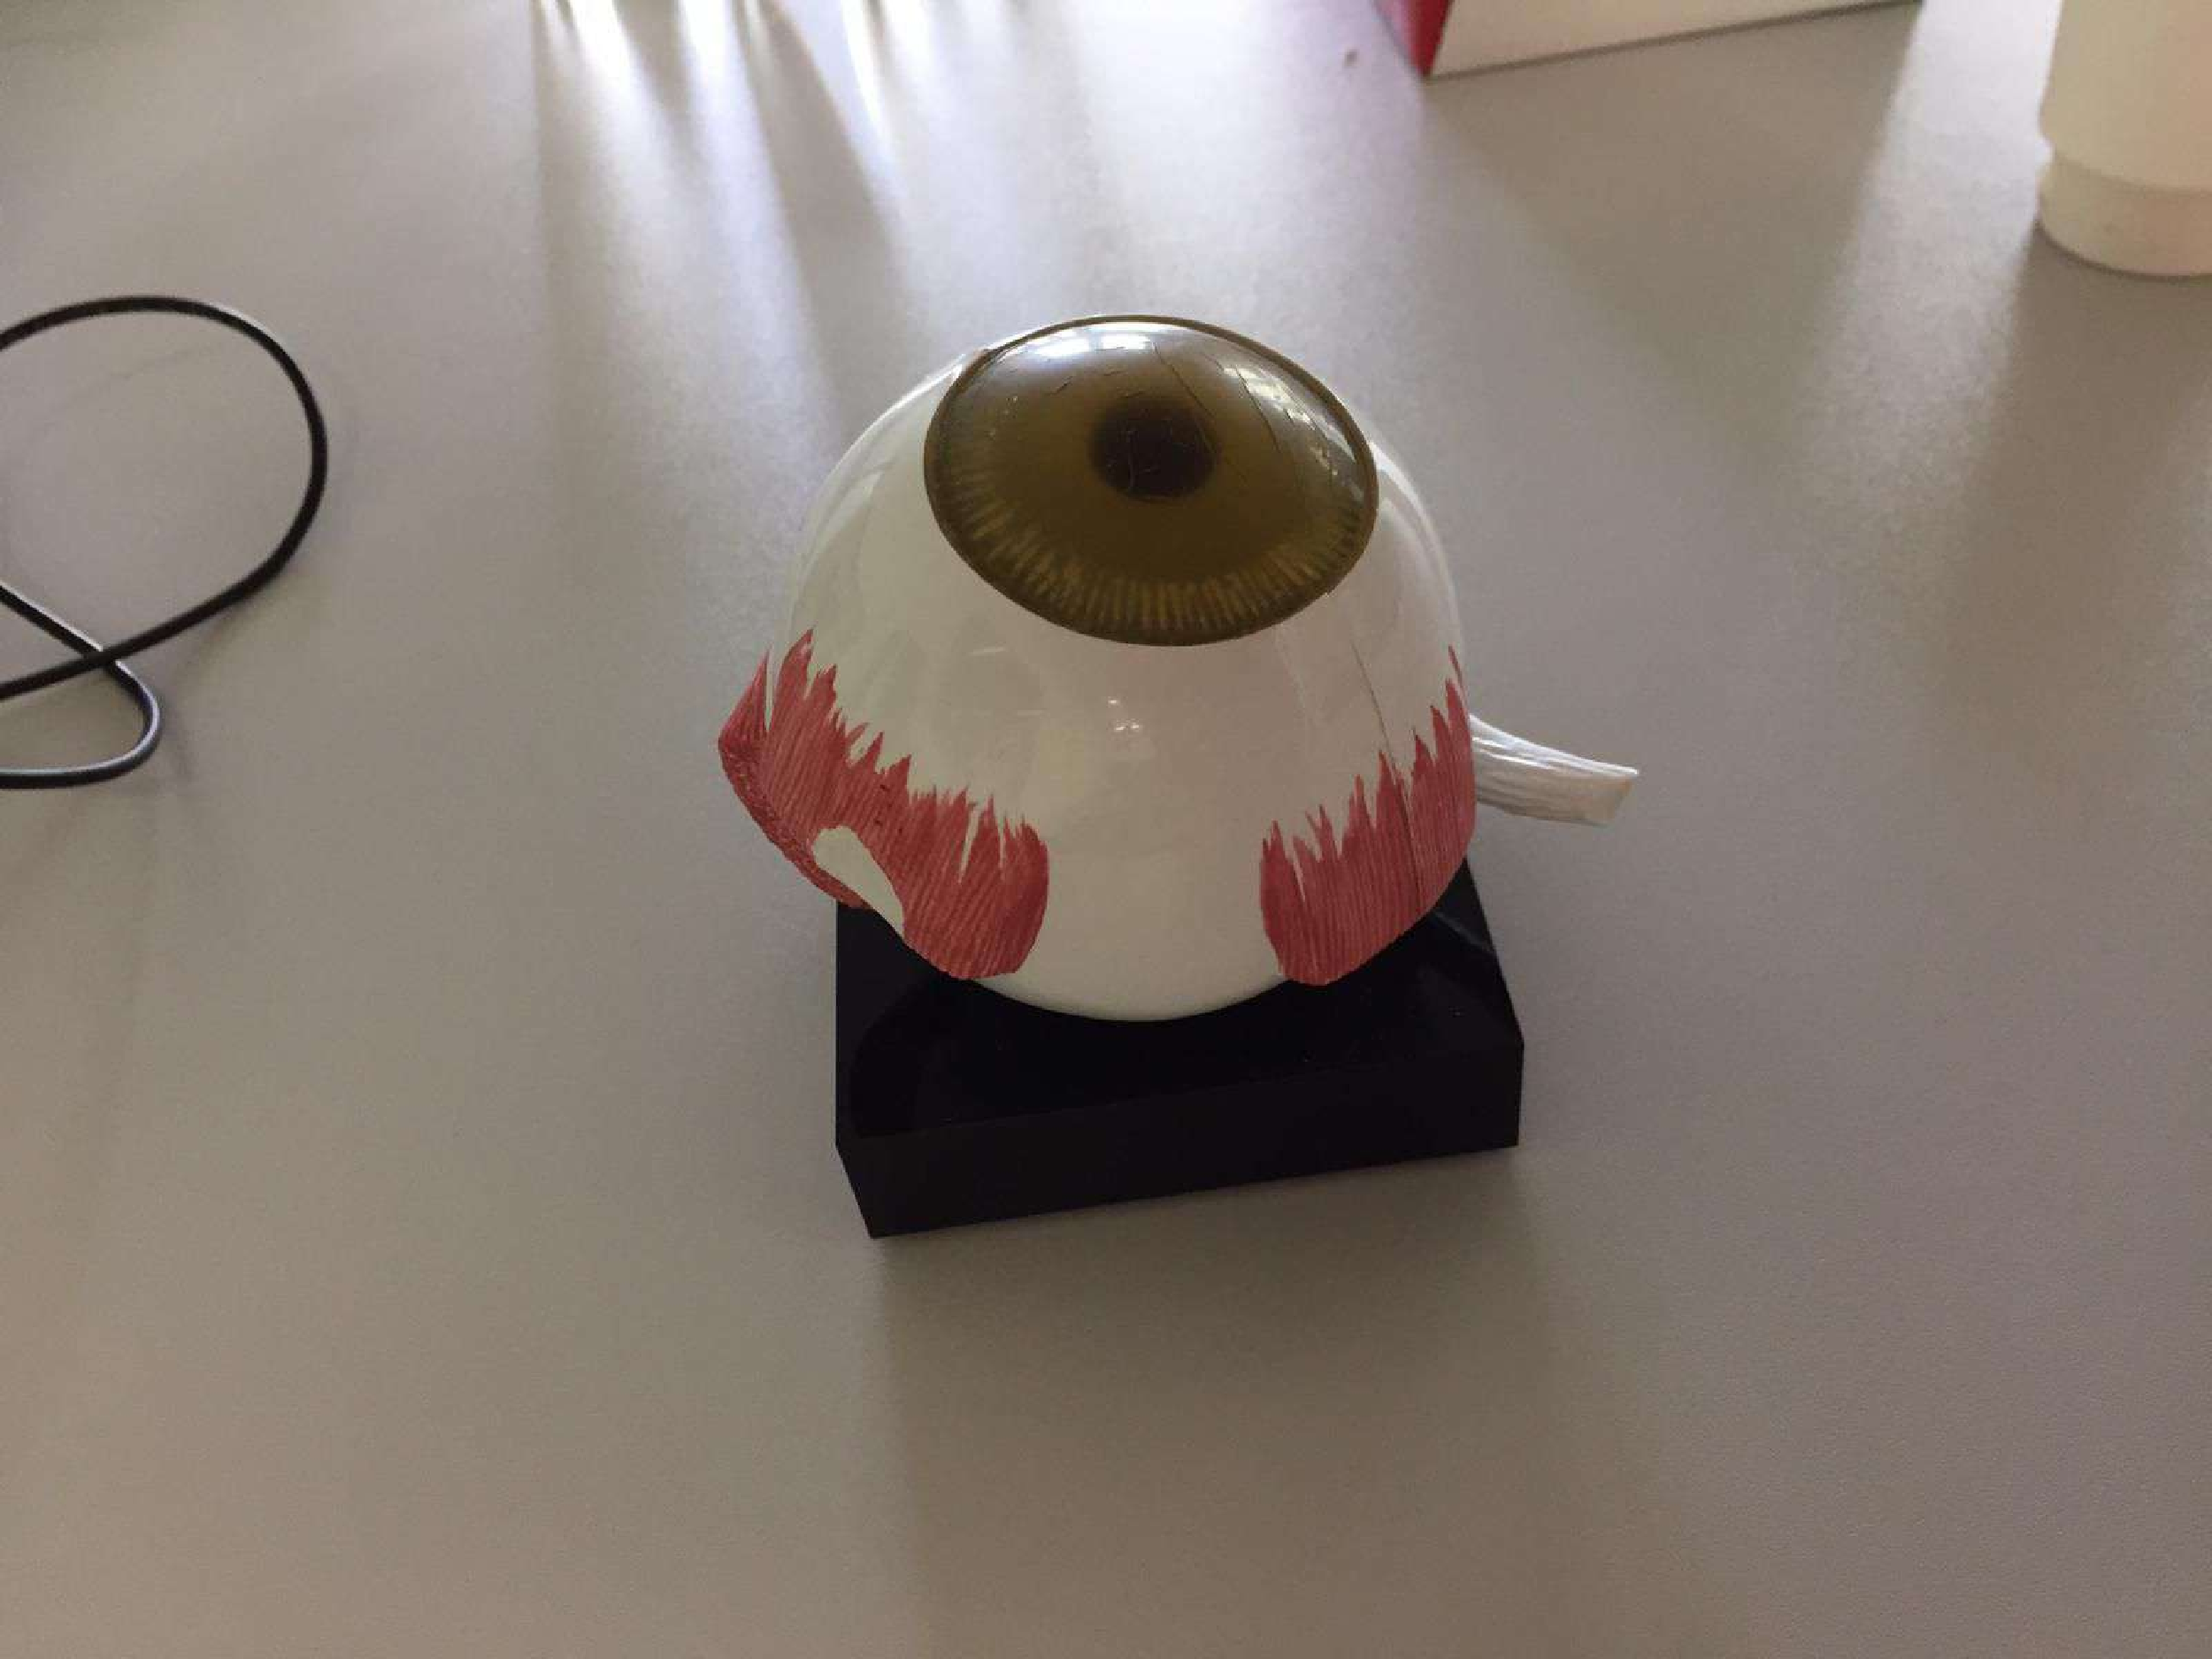
\includegraphics[width=\textwidth]{content/auge.pdf}
    \caption{Das Augenmodell.}\cite{anleitung}
    \label{fig:auge}
\end{figure}